\chapter{Geometry of the Expanding Universe}

These notes follow Leonard Susskind's first lecture on cosmology closely. The surviving transcript, together with selected blackboard frames preserved through LazyingArt LLC and Video2Book, lets us keep not only the main formulas but also the order in which the geometric ideas are introduced. The point of the lecture is deliberately narrow: we begin with expanding-universe geometry and postpone dynamics, Newtonian cosmology, and the full Friedmann--Robertson--Walker synthesis to later chapters. The mathematical thread is simple and powerful: first we convert comoving labels into physical distance, then we derive Hubble's law, then we translate that kinematics into a spatial metric, and only after that do we pass to spacetime geometry.

\section{Geometry First, Dynamics Later}

Susskind begins by refusing the usual historical prelude. We are not going to reconstruct the entire history of cosmology before getting started. We go straight to the expanding universe and to its geometry. That choice matters, because it explains why the lecture opens with idealized lines, grids, and metrics rather than with Einstein's equations or Friedmann dynamics.

What we need first is a language in which changing distances can be described cleanly. Dynamics will eventually tell us why the scale factor grows, shrinks, or does something more complicated. But before asking what determines the function \(a(t)\), we want to know what \(a(t)\) means.

\section{Comoving Coordinates and the One-Dimensional Expanding Line}

We begin with the simplest possible space: a one-dimensional line. Imagine galaxies embedded in that line and, for the moment, equally spaced. The simplification is drastic, but it isolates the essential point. We now assign a coordinate \(x\), with the understanding that \(x\) is not yet a measured distance. It is a name attached to a galaxy.

\begin{figure}
\centering
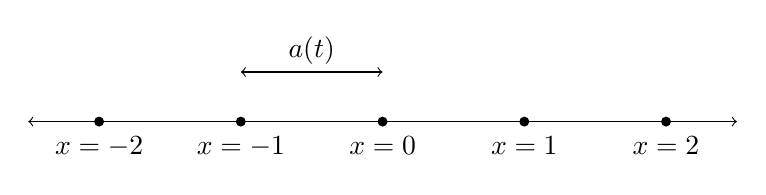
\begin{tikzpicture}[scale=0.9]
\draw[<->] (-5,0) -- (5,0);
\foreach \x/\lab in {-4/-2,-2/-1,0/0,2/1,4/2}{
  \fill (\x,0) circle (2pt);
  \node[below] at (\x,-0.08) {$x=\lab$};
}
\draw[<->] (-2,0.7) -- (0,0.7);
\node at (-1,1.0) {$a(t)$};
\end{tikzpicture}
\caption{A one-dimensional universe of equally spaced galaxies. The coordinate \(x\) labels galaxies; the neighboring physical separation is the scale factor \(a(t)\).}
\end{figure}

If the distance from the galaxy called \(x=0\) to the galaxy called \(x=1\) is \(a\), then the distance between any two galaxies is the coordinate difference multiplied by this common spacing:
\begin{equation}
d=a\,\Delta x.
\end{equation}
This is the first essential move of the lecture. The physical distance \(d\) is not \(\Delta x\). The coordinate difference only tells us which pair of galaxies we are talking about; the scale factor converts that label difference into actual geometry.

The line is now imagined as elastic. If it is stretched or contracted, the labels stay attached to the galaxies, but the physical spacing changes. In other words, \(a\) becomes a function of time:
\begin{equation}
d(t)=a(t)\,\Delta x.
\end{equation}
Homogeneity, at this stage, means only that neighboring galaxies are equally spaced everywhere along the line. The spacing itself may still change with time.

\section{From the Scale Factor to Hubble's Law}

Now we calculate the rate at which the distance between two fixed galaxies changes. The key word is fixed: we choose two galaxies and keep talking about those same galaxies, so \(\Delta x\) does not depend on time. Differentiating \(d=a\,\Delta x\) gives
\begin{align}
\dot d &= \dot a\,\Delta x \\
       &= \frac{\dot a}{a}\,a\,\Delta x \\
       &= \frac{\dot a}{a}\,d.
\end{align}
This is Hubble's law in its clean geometric form. If we define
\begin{equation}
H(t)\equiv \frac{\dot a}{a},
\end{equation}
then
\begin{equation}
\dot d = H(t)\,d.
\end{equation}

Susskind follows usage and speaks of the Hubble constant, but he immediately warns that the name is misleading. The quantity is constant in space, not in time. It is the same everywhere in a homogeneous universe, but in general it changes as the universe evolves. So it is better to think of \(H(t)\) as the Hubble parameter.

This formula already contains the striking observational point: the farther away a galaxy is, the faster it recedes. But nothing in the argument singles out a center. The law concerns the relative separation of any pair of galaxies. Every observer sees the same pattern. That is why an expanding universe need not be an explosion from one distinguished point.

The lecture then turns outward toward observation. If galaxies are moving apart, the light they exchange is redshifted. The larger the recession speed, the larger the redshift. In that way spectral lines provide a practical handle on velocity, while size and brightness provide a rough handle on distance. Hubble's original plot was not a perfect straight line at all; it was noisy. But the linear principle was there, and the geometric explanation is simpler than the observational history.

One important warning is flagged and deferred: if \(d\) is large enough, the formula \(\dot d = H d\) predicts recession speeds larger than the speed of light. Susskind does not resolve that point yet, but he emphasizes that it will matter later.

\subsection{Question \& Answer}

\paragraph{Question.} Does \(v=Hd\) mean that a given pair of galaxies must be accelerating, simply because the distance \(d\) is increasing?

\paragraph{Answer.} No. The law tells us how velocity varies with distance at a fixed time. It does not by itself tell us how the velocity of one fixed pair varies with time. That depends on the function \(a(t)\).

If
\begin{equation}
a(t)=\alpha t,
\end{equation}
then neighboring galaxies separate with constant speed \(\dot a=\alpha\). For a fixed pair,
\begin{equation}
\dot d = \alpha\,\Delta x,
\end{equation}
so their recession speed is constant in time.

If instead
\begin{equation}
a(t)=\beta t^2,
\end{equation}
then
\begin{equation}
\dot d = 2\beta t\,\Delta x,
\end{equation}
which increases with time: now the recession is accelerating.

And if
\begin{equation}
a(t)=\gamma \log t,
\end{equation}
then
\begin{equation}
\dot d = \frac{\gamma}{t}\,\Delta x,
\end{equation}
which decreases with time: the recession is decelerating.

So the Hubble law is always a statement about distance dependence. Whether a particular pair speeds up or slows down is a separate question, controlled by the detailed time dependence of \(a(t)\).

\section{Higher Dimensions, Isotropy, and Homogeneity}

There is nothing peculiarly one-dimensional about the preceding argument. We can repeat it in two dimensions by placing galaxies at the corners of a square grid and attaching to each galaxy a pair of labels \((x,y)\). Again the coordinates are comoving labels, not physical distances.

\begin{figure}
\centering
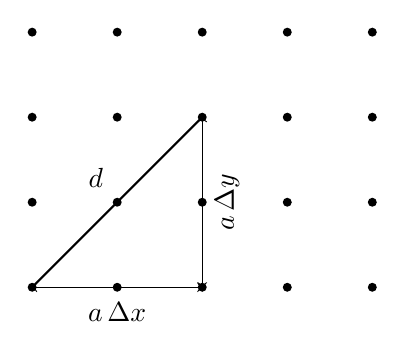
\begin{tikzpicture}[scale=0.9]
\foreach \x in {0,1,2,3,4}{
  \foreach \y in {0,1,2,3}{
    \fill (1.2*\x,1.2*\y) circle (1.8pt);
  }
}
\draw[<->] (0,0) -- (2.4,0);
\node at (1.2,-0.35) {$a\,\Delta x$};
\draw[<->] (2.4,0) -- (2.4,2.4);
\node[rotate=90] at (2.75,1.2) {$a\,\Delta y$};
\draw[thick] (0,0) -- (2.4,2.4);
\node at (0.9,1.55) {$d$};
\end{tikzpicture}
\caption{A two-dimensional comoving grid. Equal neighboring spacings in the \(x\)- and \(y\)-directions encode isotropy in this idealized model.}
\end{figure}

If neighboring galaxies are separated by the same scale factor \(a\) in both coordinate directions, then the physical legs are \(a\,\Delta x\) and \(a\,\Delta y\), and the Pythagorean theorem gives
\begin{equation}
d=a\sqrt{(\Delta x)^2+(\Delta y)^2}.
\end{equation}
In three dimensions the extension is immediate:
\begin{equation}
d=a\sqrt{(\Delta x)^2+(\Delta y)^2+(\Delta z)^2}.
\end{equation}
For a fixed pair of galaxies, the coordinate differences are constant, so differentiation again yields
\begin{equation}
\dot d=\frac{\dot a}{a}\,d.
\end{equation}
The same Hubble law survives unchanged.

At this point the lecture uses geometry to motivate two central cosmological ideas. Homogeneity means sameness from place to place. Isotropy means sameness from direction to direction. They are not identical concepts. One may imagine a universe that looks the same at every point but carries a preferred direction, so homogeneity does not by itself imply isotropy. But the observed large-scale sky is approximately the same in every direction, and that observational symmetry is what motivates using the same scale factor in the \(x\)-, \(y\)-, and \(z\)-directions.

The lecture is careful here. The universe is not exactly homogeneous or isotropic on small scales. The Milky Way already breaks exact isotropy in the sky, and any individual galaxy is obviously a local inhomogeneity. The cosmological claim is only that after averaging over sufficiently large scales, the large-scale distribution becomes approximately uniform.

\section{Why the Scale Factor Is a Bookkeeping Device, and Why the Metric Matters}

Once \(H=\dot a/a\) has appeared, the next natural question is whether the absolute size of \(a\) means anything. Susskind's answer is no, not by itself. The scale factor is partly a bookkeeping device. We may redefine it by a constant multiple without changing the physical Hubble law. If we choose a new scale factor \(b\) by
\begin{equation}
b=3a,
\end{equation}
then
\begin{equation}
\frac{\dot b}{b}=\frac{3\dot a}{3a}=\frac{\dot a}{a}.
\end{equation}
What matters physically is not the overall normalization of \(a\), but ratios involving \(a\), and in particular the ratio \(\dot a/a\). This is why the equations naturally organize themselves around such ratios.

The lecture now changes register. We have spoken about changing distances, but geometry is more naturally expressed through a metric. For neighboring points we replace \(\Delta x\) by \(dx\), and the physical distance becomes
\begin{equation}
ds=a\,dx.
\end{equation}
Therefore
\begin{equation}
ds^2=a^2\,dx^2.
\end{equation}
For the one-dimensional spatial metric, the coefficient of \(dx^2\) is simply
\begin{equation}
g_{xx}=a^2.
\end{equation}
Thus an expanding universe is already visible at the level of spatial geometry: the metric coefficient itself depends on time.

\subsection{Question \& Answer}

\paragraph{Question.} Is \(dx\) a physical distance, or only a comoving label?

\paragraph{Answer.} It is only a comoving label interval. The physical distance is \(ds=a\,dx\). One can even decide, by convention, where to place the units of distance: in \(x\), in \(a\), or shared between them. The lecture chooses to put the units into \(a\). What is not conventional is the product \(a\,dx\), and what is especially robust is the ratio \(\dot a/a\).

This is the same point in slightly different language: the coordinate mesh follows the galaxies. As the universe expands, the coordinate difference between two chosen galaxies stays fixed, while the physical distance between them changes.

Now we pass from the geometry of space to the geometry of spacetime. If the spatial separation contributes \(a^2\,dx^2\), then the proper-time interval takes the form
\begin{equation}
d\tau^2 = dt^2 - a^2(t)\,dx^2.
\end{equation}
For an observer comoving with a galaxy, \(dx=0\), and the proper time is just the ordinary time \(t\). For an object moving through the comoving grid, the spatial piece subtracts from \(dt^2\), as usual in relativity.

The blackboard frame below is especially useful because it shows the lecture's progression on the board itself: spacetime sketch at left, line element in the middle, metric notation at right.

\begin{figure}
\centering

\includegraphics[width=0.82\textwidth]{lecture_01_figure_02.png}

\vspace{1em}

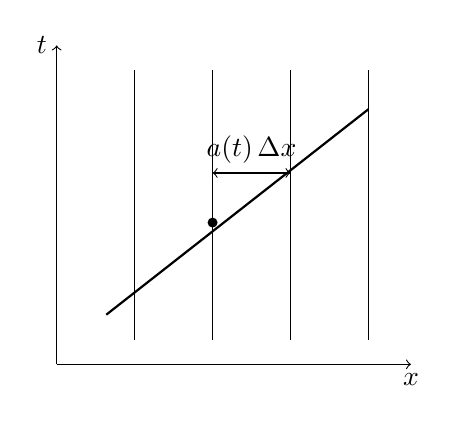
\begin{tikzpicture}[scale=0.9]
\draw[->] (0,0) -- (0,4.5);
\node[left] at (0,4.5) {$t$};
\draw[->] (0,0) -- (5.0,0);
\node[below] at (5.0,0) {$x$};

\foreach \x in {1.1,2.2,3.3,4.4}{
  \draw (\x,0.35) -- (\x,4.15);
}

\draw[thick] (0.7,0.7) -- (4.4,3.6);
\fill (2.2,2.0) circle (2pt);

\draw[<->] (2.2,2.7) -- (3.3,2.7);
\node[above] at (2.75,2.7) {$a(t)\,\Delta x$};
\end{tikzpicture}
\caption{Expanding-universe spacetime sketch and line element. The lecture frame is kept as visual evidence for the board layout, while the redraw isolates the comoving worldlines and the spatial separation at fixed time.}
\end{figure}

In three spatial dimensions, the cleaned line element suggested by the lecture and partially visible on the board is
\begin{equation}
d\tau^2 = dt^2 - a^2(t)\bigl(dx^2+dy^2+dz^2\bigr).
\end{equation}
Likewise, the matrix on the board is partly obscured, so the clean diagonal form should be read as a cautious standard completion rather than as a fully legible transcription:
\begin{equation}
g_{\mu\nu}=\mathrm{diag}\bigl(1,-a^2,-a^2,-a^2\bigr).
\end{equation}
The absence of off-diagonal \(dt\,dx\)-type terms is part of the ansatz: space and time are not mixed in this simple cosmological metric.

Susskind also pauses to note that the coefficient of \(dt^2\) being equal to \(1\) is, in this setting, largely a matter of time parametrization. If that coefficient depended only on time, one could absorb it into a redefinition of the time variable. Similarly, he takes units with \(c=1\), so one light year per year is the speed of light. But none of that changes the central geometric point: expansion is encoded by the time dependence of the spatial components of the metric.

We stop short of dynamics. One could now place this metric into Einstein's equations and ask what kind of energy-momentum tensor would produce it, but the lecture explicitly postpones that question.

\section{What We Know, What We Assume, and What the Horizon Hides}

Once the metric has been written down, the lecture widens the frame again. Homogeneity and isotropy are powerful simplifications, but they are not revealed truths. They are empirical claims, and like all empirical claims they are scale dependent.

\subsection{Question \& Answer}

\paragraph{Question.} What exactly do homogeneity and isotropy buy us in the metric?

\paragraph{Answer.} Homogeneity says that the metric coefficients do not depend on spatial position. Isotropy says that the different spatial directions are treated equally. In the metric above, the fact that the coefficients do not depend on \(x\), \(y\), or \(z\) is the metric statement of homogeneity, while the equality of the three spatial coefficients is the metric statement of isotropy.

The lecture then refines the relation between the two ideas. Isotropy about every point implies homogeneity. But homogeneity alone need not imply isotropy. One may imagine a universe filled everywhere with arrows all pointing in the same direction: every place is the same, but there is still a preferred direction.

The observational caveat is equally important. The universe is not homogeneous on the scale of galaxies, or rooms, or even modest astronomical distances. It is only after averaging over very large scales that the sky becomes approximately uniform. Susskind's analogy is a farmer's field: on one scale it looks homogeneous, on a very small scale it does not, and on a scale larger than the whole field it again fails to look homogeneous.

Then comes the horizon. The observable universe is only a finite portion of the whole. Indeed, the lecture emphasizes something stronger: the universe is larger than the part we can now see, and larger than the part we can ever see in principle. Beyond the horizon we do not know whether homogeneity and isotropy continue to hold. We may suspect they do not, but the horizon is an ultimate barrier to direct observation.

This is why the cosmological principle is both indispensable and provisional. It is an extraordinarily successful working hypothesis on the scales available to astronomy, and at the same time it is not a dogma that geometry itself enforces everywhere.

\section{Closed and Bounded Universes: The Circle Model}

The last part of the lecture asks whether the universe might be bounded. A line segment or a cube with walls is the wrong kind of boundedness, because such models violate homogeneity and isotropy. Near a wall the universe looks different than it does far from the wall. In a cube, even the observer at the center sees different things in different directions.

The right idea is bounded without boundary. The lecture first invokes the surface of a sphere as the familiar example: every place on a featureless sphere is like every other place, and every direction in the tangent surface looks the same. But to keep the algebra simple, Susskind then reduces the construction to one dimension: a closed universe that is a circle.

In one dimension, isotropy means simply that left and right are equivalent. A circle has that property, at least on scales large compared with the spacing of individual galaxies. The natural coordinate is not \(x\) but the angle \(\theta\), measured in radians. One may choose some galaxy as \(\theta=0\), and every other galaxy is labeled by an angle. The periodicity \(\theta\sim \theta+2\pi\) expresses the closed nature of the space.

The lecture then makes the crucial identification. If we draw the one-dimensional universe as a circle of radius-like parameter \(a\), the total distance around it is
\begin{equation}
L = 2\pi a.
\end{equation}
For a small angular separation \(\Delta\theta\), the physical distance along the circle is
\begin{equation}
d=a\,\Delta\theta.
\end{equation}
So for neighboring points,
\begin{equation}
ds^2=a^2\,d\theta^2.
\end{equation}
This formula is not visibly written on the captured blackboard frame, but it is the clean mathematical form supported by the lecture's spoken derivation.

\begin{figure}
\centering

\includegraphics[width=0.82\textwidth]{lecture_01_figure_03.png}

\vspace{1em}

\begin{tikzpicture}[scale=1.0]
\draw (0,0) circle (2.3);
\draw[->] (1.4,1.8) arc[start angle=52,end angle=74,radius=2.3];
\fill (2.3,0) circle (2pt);
\node[right] at (2.3,0) {$\theta=0$};
\fill (1.72,1.52) circle (2pt);
\node[right] at (1.82,1.55) {$\theta$};
\draw (0,0) -- (2.3,0);

\draw (-4.2,2.2) -- (-1.8,2.2);
\node[below] at (-3.0,2.2) {$2\pi a$};
\end{tikzpicture}
\caption{The closed one-dimensional universe as a circle. The lecture frame is kept because the board layout itself motivates the reconstruction: angular labels on the right and an unwrapped circumference cue \(2\pi a\) on the left.}
\end{figure}

The similarity with the straight-line model is immediate. If \(a\) depends on time, then
\begin{equation}
d(t)=a(t)\,\Delta\theta,
\end{equation}
and differentiation gives
\begin{align}
\dot d &= \dot a\,\Delta\theta \\
       &= \frac{\dot a}{a}\,d.
\end{align}
So Hubble's law survives in the closed universe as well, at least for separations small enough that we do not worry about the alternative route around the other side of the circle.

The spacetime metric of the time-dependent circle model is therefore
\begin{equation}
d\tau^2 = dt^2 - a^2(t)\,d\theta^2.
\end{equation}
The lecture then draws the resulting spacetime as a family of circles stacked in time. If \(a\) grows, the circles widen. If it later shrinks, the surface narrows again. Extrinsically, the picture resembles a cylinder, a cone, or a vase-like surface, depending on the choice of \(a(t)\).

\begin{figure}
\centering
\begin{tikzpicture}[scale=0.9]
\draw (-6,0) ellipse (0.8 and 0.22);
\draw (-6.8,0) -- (-6.8,3.2);
\draw (-5.2,0) -- (-5.2,3.2);
\draw (-6,3.2) ellipse (0.8 and 0.22);
\node at (-6,-0.6) {$a=\text{const}$};
\node at (-6,-1.0) {cylinder};

\draw (-0.9,0.12) -- (0,3.2);
\draw (0.9,0.12) -- (0,3.2);
\draw (0,0.12) ellipse (0.9 and 0.22);
\node at (0,-0.6) {$a\propto t$};
\node at (0,-1.0) {cone};

\draw (5.1,0.15) .. controls (3.9,0.9) and (4.4,2.4) .. (5.2,3.2);
\draw (6.9,0.15) .. controls (8.1,0.9) and (7.6,2.4) .. (6.8,3.2);
\draw (6.0,0.15) ellipse (0.9 and 0.22);
\draw (6.0,3.2) ellipse (0.8 and 0.20);
\node at (6,-0.6) {$a=a(t)$};
\node at (6,-1.0) {``vase''};

\draw[->] (-8.3,0) -- (-8.3,3.5);
\node[left] at (-8.3,3.5) {$t$};
\end{tikzpicture}
\caption{Explanatory redraw of the circle-universe spacetime for three choices of scale factor. These are external visualization aids for the lecture's geometry, not intrinsic definitions of curvature by themselves.}
\end{figure}

\subsection{Question \& Answer}

\paragraph{Question.} Where did the Big Bang happen, and what do the cylinder and cone pictures really mean?

\paragraph{Answer.} In this model the Big Bang does not happen at one preferred place in some external space. If \(a(t)\to 0\), then every separation \(a(t)\,\Delta\theta\) tends to zero. The whole closed universe shrinks everywhere at once. So the answer to ``Where did it happen?'' is: everywhere.

This is exactly why the lecture insists that cosmic expansion is not like a bomb exploding in a room. The galaxies are not being ejected from one point into pre-existing space. Rather, the geometry itself changes, and with it the distances between all comoving points.

As for curvature, the embedding picture can mislead. If \(a\) is constant, the spacetime picture is a cylinder. In the one-space, one-time toy model of the lecture, that cylinder is flat: one can cut it open and lay it out on a plane without stretching it. If \(a\propto t\), the picture is a cone. A cone is also flat except at its tip, where there is a conical singularity. Thus the tip represents a special spacetime event, while the spatial universe at any fixed time is still the closed circle.

The moral is twofold. First, the Big Bang is an everywhere-event in the geometry, not an explosion from a favored point. Second, curvature is an intrinsic question; one must not read it naively from the way a picture is embedded in a higher-dimensional drawing space.

\section{Summary}

The lecture builds cosmology from the bottom up. We begin with comoving labels, discover that physical distance is \(d=a\,\Delta x\), differentiate to obtain Hubble's law \(\dot d=(\dot a/a)d\), and then recognize that the same scale factor is the coefficient in the spatial metric. Expansion is therefore not an extra story added on top of geometry; it is the statement that the spatial part of the metric depends on time.

Homogeneity and isotropy justify using one common scale factor on large scales, though only as empirical approximations within the observable universe. Finally, the circle model shows how a universe can be closed and bounded without boundary, while still obeying a local Hubble law. That closes the lecture's geometric arc: the Big Bang is not matter blasted from one point into space, but rather space itself changing its scale everywhere at once.